\index{general}{$P_1\times P_0$}
\begin{flushright} {\tiny {\color{gray} \tt  pair\_p1p0.tex}} \end{flushright}
%~~~~~~~~~~~~~~~~~~~~~~~~~~~~~~~~~~~~~~~~~~~~~~~~~~~~~~~~~~~~~~~~~~~~~~~~~~~~~~~~~~~~~~~~~~~~~~~~~~

The standard form of the ${\bm P}_1 \times P_0$ element is as follows:
\begin{verbatim}
*          
|\   P1      |\    P0
| \          | \
|  \         |  \
|   \        |   \
|    \       |    \
|     \      |  o  \
|      \     |      \
*-------*    ---------
\end{verbatim}
The pressure is constant inside the element and discontinuous from element 
to element.

\textcite{qizh07b} (2007) state: 
\begin{displayquote}
{\color{darkgray}
The element is unstable for any mesh since
the dimension of the discrete velocity space is always less than that of the pressure space (with
Dirichlet boundary condition).
However, this element provides optimal approximations for both
the velocity and the pressure on many mesh families.} 
\end{displayquote}

\begin{center}
\fbox{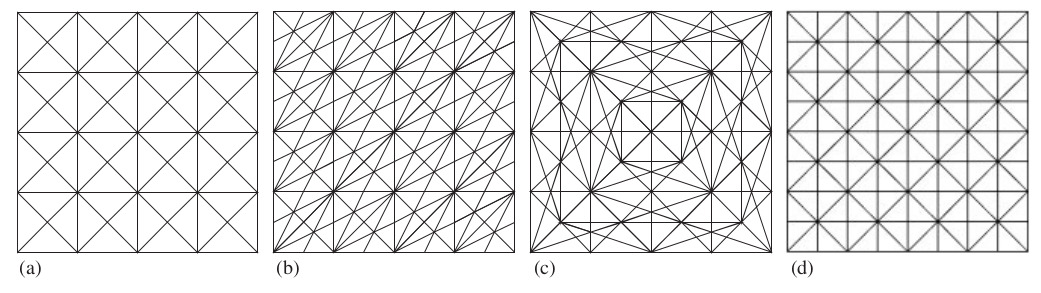
\includegraphics[width=12cm]{images/pair_p1p0/qizh07}}\\
{\captionfont A crisscross, a Powell–Sabin, a Powell–Sabin–Heindl and a type-2 grid.
Taken from \cite{qizh07}.}
\end{center}
\index{general}{Powell-Sabin-Heindl grid}

\textcite{arno93} (1993) states: 
\begin{displayquote}
{\color{darkgray}
Unfortunately, this simplest possible Stokes element is notoriously unstable. On any 
triangulation with at least three vertices on the boundary the dimension of the pressure
space exceeds that of the velocity space [...] and the finite
dimensional problem is singular. 
Moreover, while the discrete velocity field $u_h$ is uniquely
determined (as it is for any conforming method for the Stokes problem), for this choice of
elements $u_h$ belongs to the space of divergence-free fields piecewise linear fields, and on
many meshes, for example on a uniform diagonal mesh of the square [...],
this space is known to reduce to zero. So even after accounting for the indeterminancy of
the pressure we have no convergence.}
\end{displayquote}

Example 3.2 of \textcite{bobf08} (2008) explain neatly the locking phenomenon and how 
to circumvent it via a so-called cross-grid macroelement. See also 
\textcite{hokl03} (2003).

Note that \textcite{zhan08} (2008) establishes the stability of the ${\bm P}_1\times P_0$
mixed-element on general Powell-Sabin triangular grids.

\begin{displayquote}
{\color{darkgray}
The piecewise linear finite element solution approximating the velocity is
divergence-free pointwise for the Stokes equations. The finite element solution approximating 
the pressure in the Stokes equations can be obtained as a byproduct if an iterative
method is adopted for solving the discrete linear system of equations. Numerical tests are
presented confirming the theory on the stability and the optimal order of convergence for
the $P_1$ Powell-Sabin divergence-free finite element method.}
\end{displayquote}

\begin{center}
\fbox{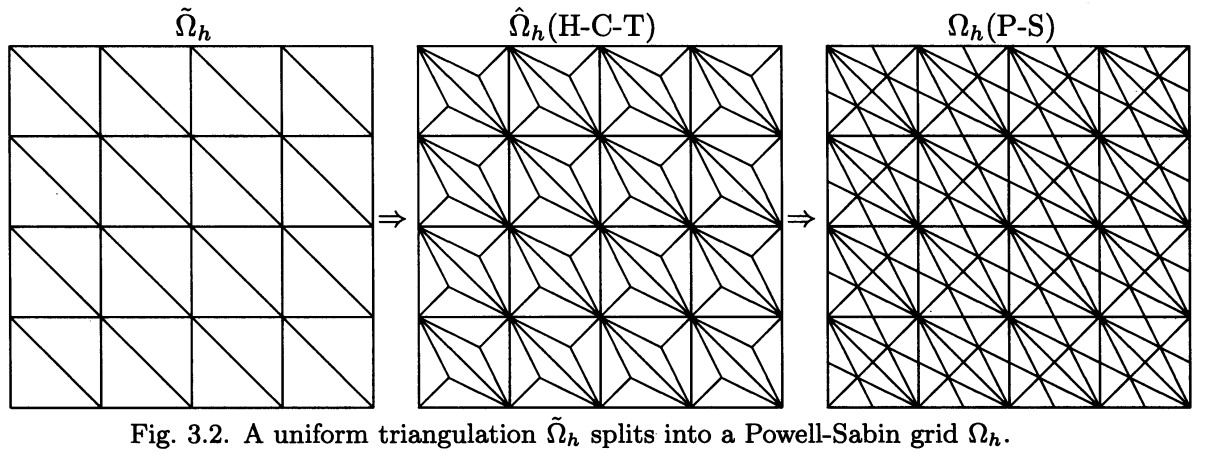
\includegraphics[width=12cm]{images/pair_p1p0/hct_ps}}\\
{\captionfont Taken from \textcite{zhan08}, 2008. Looking at this node layout we see that 
this element pair will not be trivial to implement since the velocity nodes inside the element
are placed like for the $P_2^+$ element but instead make up 6 smaller elements.}
\end{center}

\begin{center}
\fbox{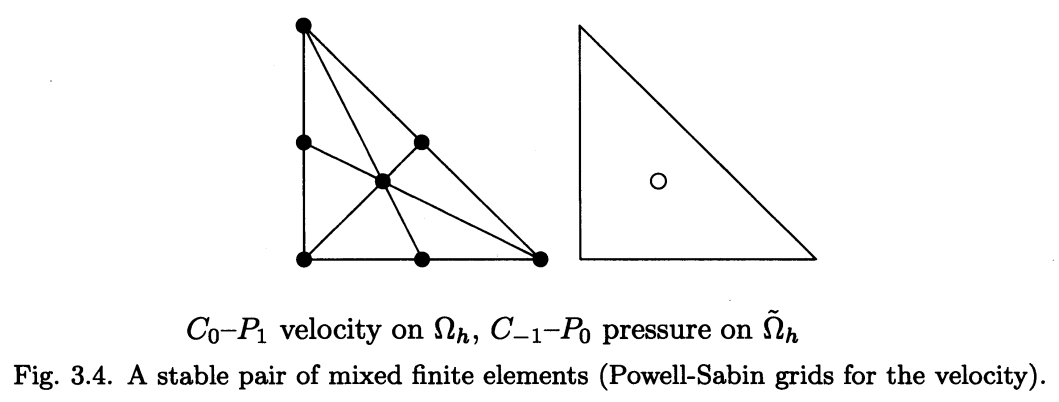
\includegraphics[width=8cm]{images/pair_p1p0/zhan08}}\\
{\captionfont Taken from \textcite{zhan08}, 2008.}
\end{center}

\index{general}{Powell-Sabin grid}
\index{general}{Hsieh-Clough-Tocher grid}

In his lecture notes\footnote{\url{https://www.math.tamu.edu/~guermond/}}, 
Guermond states 
\begin{displayquote}
{\color{darkgray}
A simple alternative to the 
$Q_1\times P_0$ element consists of using the $P_1\times P_0$ element.
Let ${\cal T}_h$  be a mesh of $D$ composed of affine simplices, and approximate the 
velocity with continuous piecewise linear polynomials and the pressure with
(discontinuous) piecewise constants. Since the velocity is piecewise linear, its
divergence is constant on each simplex. As a result, testing the divergence
of the velocity with piecewise constants enforces the divergence to be zero
everywhere. That is to say, the $P_1\times P_0$ finite element yields a velocity 
approximation that is exactly divergence-free [...]. Unfortunately,
this pair does not satisfy the inf-sup condition.}
\end{displayquote}

I have not found a paper yet which showcases its accuracy on a manufactured solution
and compares it to other element pairs.


\begin{center}
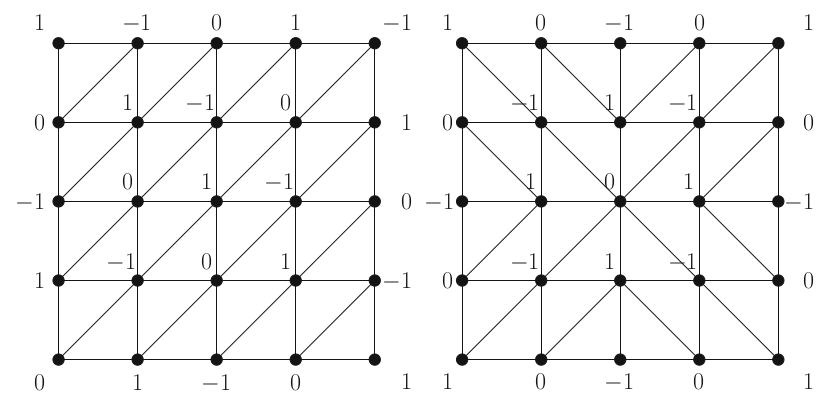
\includegraphics[width=10cm]{images/pair_p1p0/john16}\\
{\captionfont Taken from \textcite{john16}, page 65.
On these meshes, $P_1$ possesses 25 degrees of freedom (number of vertices) whereas $P_0$ has
even 32 degrees of freedom (number of mesh cells). There is one degree of freedom
less in the corresponding pressure finite element spaces since the discrete pressure
has to fulfill the integral mean value condition. Thus, spurious modes have to be
expected.
}
\end{center}



Elman Silvester Wathen say (5.3.3) that 
\begin{displayquote}
{\color{darkgray}
It can be readily stabilized using the pressure jump
stabilization together with an appropriate macroelement subdivision.}
\end{displayquote}
See \textcite{nosi98} (1998) for globally and locally stabilised versions.

In \textcite{caod86} (1986), we read\footnote{page 138}:
\begin{displayquote}
{\color{darkgray}
Another interesting choice is the triangle with linear velocity and 
piecewise-constant pressure.
The vertices of the triangle are velocity nodes
and the element centroids may be taken as pressure nodes.
This element element would appear to be the simplest and most natural choice
for a mixed method, but again the consistency condition fails.
An easy physical interpretation is possible in this case:
As $h\rightarrow 0$ the number of triangles increases faster than the number
of vertices. Concequently, the dimension of the pressure space $P^h$
grows to exceed that of the velocity space $V^h$.
For example, consider the unit square with an $N\times N$ rectangular mesh
subdivided into $2N^2$ triangles. We have $2N^2$ pressure nodes
(and basis functions) but only $2(N-1)^2$ interior velocity degrees of freedom
(and basis functions) if Dirichlet data is specified. 
Each pressure equation is a discrete constraint equation, and the 
problem is overconstrained. The velocity $\vec{\upnu}_h=\vec{0}$, which 
satisfies the mass constraint but not the momentum equations.

[..]

A balance between the dimensions of the velocity and pressure spaces
should be maintained as the mesh size $h$ decreases.
That is, if the dimension of the pressure space $P^h$ is too large
relative to that of the velocity space as the mesh is refined,
the discrete constraint equations dominate the discrete momentum equations.
It has been argued from this standpoint that elements should 
be chosen such that $dim\; P^h < dim\; V^h$. 
While the underlying reasoning is plausible and this gives a good 
guideline to follow in practice, it is neither necessary nor sufficient.
In fact the inf-sup condition provides a mathematical theory 
for selecting elements.  
}
\end{displayquote}
 

 
